\documentclass[11pt]{article}

\usepackage{fullpage,times}%charter}
\usepackage{color}

\usepackage{tikz}
\usetikzlibrary{arrows.meta}
\usetikzlibrary{automata}
%% macros
\newcommand{\ax}[1]{\texttt{AX}(#1)}
\newcommand{\ex}[1]{\texttt{EX}(#1)}
\newcommand{\af}[1]{\texttt{AF}(#1)}
\newcommand{\ef}[1]{\texttt{EF}(#1)}
\newcommand{\ag}[1]{\texttt{AG}(#1)}
\newcommand{\eg}[1]{\texttt{EG}(#1)}
\newcommand{\au}[2]{\texttt{A}(#1\ \texttt{U}\ #2)}
\newcommand{\eu}[2]{\texttt{E}(#1\ \texttt{U}\ #2)}
\newcommand{\sem}[1]{[\!\![#1]\!\!]}

\newcommand{\euntil}[3]{\texttt{E}(#1\ \texttt{U}^{#3}\ #2)}
\newcommand{\auntil}[3]{\texttt{A}(#1\ \texttt{U}^{#3}\ #2)}


\newcommand{\lx}[1]{\texttt{X}(#1)}
\newcommand{\lf}[1]{\texttt{F}(#1)}
\newcommand{\llg}[1]{\texttt{G}(#1)}
\newcommand{\lu}[2]{(#1\ \texttt{U}\ #2)}

\newcommand{\sol}[1]{{\color{blue}#1}}
%\newcommand{\sol}[1]{}
\begin{document}

\hrule
\smallskip

\noindent

\noindent
You can review the latex source for this assignment-file to
learn and use latex to prepare your homework submission. You will see
the use of macros (to write uniformly formatted text), different
text-styles (emphasized, bold-font), different environments (figures,
enumerations).

It is not required that you use exactly this latex source to prepare
your submission. 
\smallskip
\hrule


\begin{center}
{\Large\bf Homework 4 (CTL/LTL/BDD): ComS/CprE/SE 412, ComS 512}

\medskip

Due-date: April 18 at 11:59PM.

\medskip


\end{center}

\noindent
\textbf{
Submit online on Canvas two files: the source file in latex format and
the pdf file generated from latex. Name your files:
$\langle\mbox{your-net-id}\rangle$-hw4.$\langle\mbox{tex/pdf}\rangle$.
}

\hrule
\noindent
\smallskip

\emph{ Homework must be individual's original work. Collaborations and
  discussions of any form with any students or other faculty members
  or soliciting solutions on online forums are not allowed. Please
  review the academic dishonesty policy on our syllabus. If you have
  any questions/doubts/concerns, post your questions/doubts/concerns
  on Piazza and ask TA/Instructor.}

\smallskip
\hrule

\begin{enumerate}

\item
  Draw the ROBDD for the following function.
  \[
  f(x_1, x_2, x_3, x_4) =
  \left\{
  \begin{array}{ll}
    1 & \mbox{if the sum of $x_i$'s is equal to even} \\
    0 & \mbox{otherwise}
  \end{array}
  \right.
  \]
  In the above, the domain of $x_i$ is $\{0, 1\}$.
\hfill (5pts)

\textbf{Answer}: The ROBDD that produces terminal node $1$ if the sum of the decision nodes is even, and otherwise 0 is depicted below. Here, the dashed line means $0$, and the solid transition means $1$.

\begin{center}
    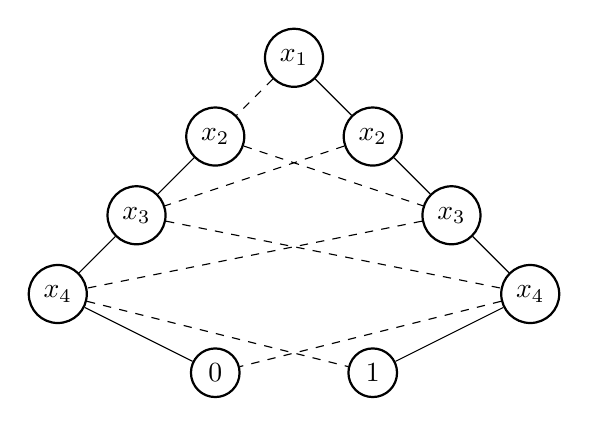
\begin{tikzpicture}

      \begin{scope}[every node/.style={circle,thick,draw}]
        \node[] (x1) at (0,0) {$x_1$};
        \node[] (x2_r) at (1,-1) {$x_2$};
        \node[] (x2_l) at (-1, -1) {$x_2$};
        \node[] (x3_r) at (2, -2) {$x_3$};

        \node[] (x3_l) at (-2, -2) {$x_3$};
        
        \node[] (x4_r) at (3, -3) {$x_4$};
        \node[] (x4_l) at (-3, -3) {$x_4$};

        \node[] (1_r) at (1, -4) {$1$};
        \node[] (0_l) at (-1, -4) {$0$};
        
      \end{scope}
      
      \begin{scope}%[>={Stealth[black]},
          %every node/.style={fill=white,circle}]
        \draw [dashed] (x1) edge (x2_l);
        \path [-] (x1) edge (x2_r);
        
        \draw [dashed] (x2_r) edge (x3_l);
        \path [-] (x2_r) edge (x3_r);
        \draw [dashed] (x2_l) edge (x3_r);
        \path [-] (x2_l) edge (x3_l);
        
        \draw [dashed] (x3_r) edge (x4_l);
        \path [-] (x3_r) edge (x4_r);
        \draw [dashed] (x3_l) edge (x4_r);
        \path [-] (x3_l) edge (x4_l);

        \path [-] (x4_r) edge (1_r);
        \draw [dashed] (x4_r) edge (0_l);
        
        \draw [dashed] (x4_l) edge (1_r);
        \path [-] (x4_l) edge (0_l);
      \end{scope}
    \end{tikzpicture}
        \end{center}

  
\item 
 Identify the states in the following Kripke structure that satisfy
  the given formula. Justify your solution.

\begin{center}
    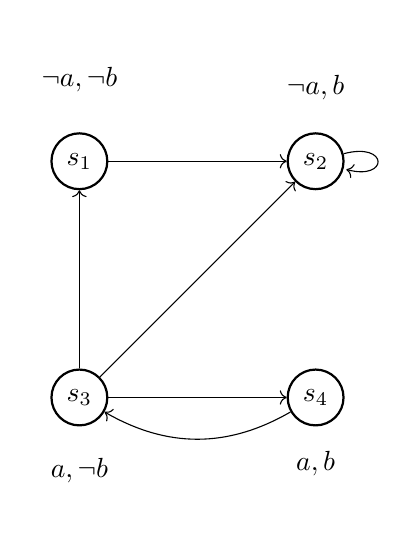
\begin{tikzpicture}

      \begin{scope}[every node/.style={circle,thick,draw}]
        \node[label={$\neg a, \neg b$}] (s1) at (0,0) {$s_1$};
        \node[label={$\neg a, b$}] (s2) at (3,0) {$s_2$};
        \node[label=below:{$a, \neg b$}] (s3) at (0, -3) {$s_3$};
        \node[label=below:{$a, b$}] (s4) at (3, -3) {$s_4$};
      \end{scope}
      
      \begin{scope}%[>={Stealth[black]},
          %every node/.style={fill=white,circle}]
        \path [->] (s1) edge (s2);
        \path [->] (s3) edge (s1);
        \path [->] (s3) edge (s2);
        \path [->] (s3) edge (s4);
        \path [->] (s2) edge[loop right] (s2);
        \path [->] (s4) edge[bend left] (s3);
      \end{scope}
    \end{tikzpicture}
        \end{center}

\begin{enumerate}
\item $\llg{a}$ 

\textbf{Answer}: $\{\}$
\item $\lu{a}{b}$ 

\textbf{Answer}: $\{s_2, s_4\}$

\item $\lu{a}{\lx{a \land \neg b}}$ 

\textbf{Answer}: $\{s_4\}$


  \item $\lx{a\land b}\ \land\ \lf{\neg a \land \neg b}$ 

  \textbf{Answer}: $\{\} $

  
    \end{enumerate}
\hfill(10pts)

\item Prove or disprove the following claims. 
\begin{enumerate}
\item $\llg{\lf{\lx{p}}}$ and $\llg{\lx{\lf{p}}}$ are equivalent.

\textbf{Answer}: As $\lf{\lx{p}}$ and $\lx{\lf{p}}$ are equivalent; therefore, it can be immediately  conferred that $\llg{\lf{\lx{p}}}$ and $\llg{\lx{\lf{p}}}$ are equivalent.

    We know two formulas become equivalent if both are satisfied in one path. Let's assume a path $s_0 s_1 s_2 s_3...s_k, ...s_{k+k}...$, where $p$ holds after each k interval, which means $s_k, s_{k+k}, ...$ satisfy $p$. 

    Here, all states starting from $s_0$ satisfy $\lf{\lx{p}}$, and similarly it also satisfies $\lx{\lf{p}}$. Therefore, we can conclude that $\llg{\lf{\lx{p}}}$ and $\llg{\lx{\lf{p}}}$ are equivalent

       
  \item $\llg{\lf{p}} \ \Rightarrow\ \llg{\lf{q}}$ and
    $\lf{\llg{\neg p}} \ \Rightarrow\ \lf{\llg{q}}$ are equivalent.

    \textbf{Answer}: 

    $\llg{\lf{p}} \ \Rightarrow\ \llg{\lf{q}}$ can be modified as $\neg \llg{\lf{p}} \lor \llg{\lf{q}} = \lf{\llg{\neg p}} \lor \llg{\lf{q}}$. Similarly, $\lf{\llg{\neg p}} \ \Rightarrow\ \lf{\llg{q}}$ can be modified as $\neg \lf{\llg{\neg p}} \lor \lf{\llg{q}} = \llg{\lf{p}} \lor \lf{\llg{q}}$. 
    Two formulas become equivalent if one is satisfied in one path and another is also satisfied in that path.  
    Let's consider the following Kripke structure with $p \in L(s_0)$ and $q \in L(s_1)$. 

        \begin{center}
    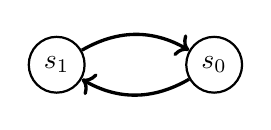
\begin{tikzpicture}

      \begin{scope}[every node/.style={circle,thick,draw}]
        \node (s0) at (0,0) {$s_0$} ;
        \node (s1) at (-2,0) {$s_1$};

      \end{scope}

      \begin{scope}[%>={Stealth[black]},
          every node/.style={fill=white,circle},
          every edge/.style={draw=black,very thick}]
        \path [->] (s0) edge[bend left, above] (s1);
        %\path [->] (s0) edge[loop left] (s0);
        \path [->] (s1) edge[bend left, below] (s0);
       % \path [->] (s1) edge[loop right] (s1);

      \end{scope}
    \end{tikzpicture}
        \end{center}
    This satisfies $\llg{\lf{p}} \ \Rightarrow\ \llg{\lf{q}}$ but it does not satisfy $\lf{\llg{\neg p}} \ \Rightarrow\ \lf{\llg{q}}$. Therefore, they are not equivalent. 

  \item Given any Kripke structure, one can verify whether a state
    satisfies the CTL formula $\af{\ag{p}}$ using the LTL formula
    $\llg{\lf{\neg p}}$. (Note that, the question is not asking
    whether the two formulas are equivalent or not).
    
\textbf{Answer}: There is no equivalent LTL formula for $\af{\ag{p}}$, because $\lf{\llg{p}}$ cannot capture the branching behavior. However, negating $\lf{\llg{p}}$ becomes $\llg{\lf{\neg p}}$. If $\llg{\lf{\neg p}}$ is satisfied, which means $\neg p$ is satisfied infinitely often, then $\af{\ag{p}}$ becomes false, and we can say that $\af{\ag{p}}$ does not hold and can verify $\af{\ag{p}}$. But if $\llg{\lf{\neg p}}$ is not satisfied, we cannot say the negation of $\llg{\lf{\neg p}}$  holds and cannot conclude $p$ is true finally globally. Therefore, $\llg{\lf{\neg p}}$ cannot be used to verify the property. 

   
  \item A state satisfies $(\ag{p}) \ \Rightarrow\ (\af{q})$ if and only
    if the state satisfies $(\llg{p}) \ \Rightarrow\ (\lf{q})$.

\textbf{Answer}: $(\llg{p}) \ \Rightarrow\ (\lf{q}) = \neg \llg{p} \lor \lf{q} = \lf{\neg p} \lor \lf{q}$. 

$(\ag{p}) \ \Rightarrow\ (\af{q}) = \neg (\ag{p}) \lor (\af{q}) = \ef{\neg p} \lor \af{q}$. 

We know a state satisfies LTL property $\phi$ iff $\forall \pi \in path(s). \pi \models \phi$. 
If a state satisfies an LTL formula $s \models \lf{\neg p} \lor \lf{q}$, it either satisfies $\lf{\neg p}$ or $\lf{q}$. Let's consider the following Kripke structure where $p \in L(s_1) \land L(s_2)$, $\neg p \in L(s_0)$. 
Here, $s_1 \models \ef{\neg p}$, but it does not satisfy $\lf{\neg p}$ because there exists one path $s_1$ to $s_1$ which satisfies $p$. As the question asks for \textbf{if and only if } condition, it should hold from both ends to satisfy the statement in the question. However, it does not; therefore, the statement in question does not hold. 

    \begin{center}
    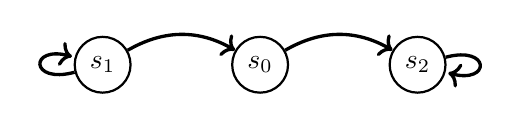
\begin{tikzpicture}

      \begin{scope}[every node/.style={circle,thick,draw}]
        \node (s1) at (-2,0) {$s_1$} ;
        \node (s0) at (0,0) {$s_0$};
        \node (s2) at (2,0) {$s_2$};

      \end{scope}

      \begin{scope}[%>={Stealth[black]},
          every node/.style={fill=white,circle},
          every edge/.style={draw=black,very thick}]
        \path [->] (s1) edge[bend left, above] (s0);
        \path [->] (s1) edge[loop left] (s1);
        \path [->] (s0) edge[bend left, below] (s2);
       \path [->] (s2) edge[loop right] (s2);

      \end{scope}
    \end{tikzpicture}
        \end{center}


% As the LTL formula $\lf{q}$ is equivalent to the CTL formula $\af{q}$, we need to prove whether a state satisfies LTL $\lf{\neg p}$, also satisfies CTL $\ef{\neg p}$.  

% If a state satisfies $\lf{\neg p} $, we can write it will satisfy the CTL formula $\af{\neg p}$. From the properties of path quantification, if all path satisfies a property, one can say that some path will also satisfy that property. Therefore, if $\af{\neg p}$ holds, we can say $\ef{\neg p}$ also holds. So, a state satisfies $(\ag{p}) \ \Rightarrow\ (\af{q})$ if and only if the state satisfies $(\llg{p}) \ \Rightarrow\ (\lf{q})$

% cannot write that it will satisfy CTL formula $\ef{\neg p}$. 
% As the existential property cannot be expressed in LTL, therefore, a state satisfying $\lf{\neg p} \lor \lf{q}$ does not mean it will satisfy any existential CTL property $\ef{\neg p} \lor \af{q}$.
       


       
  \item A state satisfies $\lu{(\neg q)}{(\neg p \land \neg q)} $ implies
    that the state satisfies $\neg \lu{p}{q}$.
    
\textbf{Answer}:

$\neg \lu{p}{q}$ can be written as $\lu{(p \land \neg q)}{(\neg p \land \neg q)} \lor \llg{p \land \neg q}$.


 Similarly, $\lu{(\neg q)}{(\neg p \land \neg q)} = \lu{(\neg q)}{\neg (p \lor q)}$. 

 We need to show $\lu{(\neg q)}{\neg (p \lor q)}  \Rightarrow \neg \lu{p}{q}$ = $\neg (\lu{(\neg q)}{\neg (p \lor q)})  \lor \neg \lu{p}{q}$ 
 
 $\neg (\lu{(\neg q)}{\neg (p \lor q)})$ holds in a state if $(p \lor q)$ holds immediately or it satisfies $q, q ...$ until it reaches  $(p \lor q)$ in all paths starting from that state.  

Here, $\neg \lu{p}{q}$ is satisfied if $\lu{p}{q}$ is not satisfied, which means $\llg{p \land \neg q}$ is satisfied. In other words, $p$ is satisfied globally. 

As $\neg (\lu{(\neg q)}{(\neg p \land \neg q)})$ is satisfied if $(p \lor q)$ holds, therefore $\lu{(\neg q)}{\neg (p \lor q)}  \Rightarrow \neg \lu{p}{q}$  holds. 

We can say that a state satisfies $\lu{(\neg q)}{(\neg p \land \neg q)} $ implies
    that the state satisfies $\neg \lu{p}{q}$.
 


\end{enumerate}
\hfill(20pts)


\item 
  Identify the LTL formulas whose semantics is represented in the language
  of the following automata. Justify your solution.
  (\emph{The start states are denoted by the states which have an incoming edge
  from the "start". The edge labels indicate a boolean formula; for instance, 
  $q_0$ on boolean formula $a$ has an edge to itself in the $A_1$)})
  \begin{enumerate}
  \item Automata $A_1$
    \begin{center}
    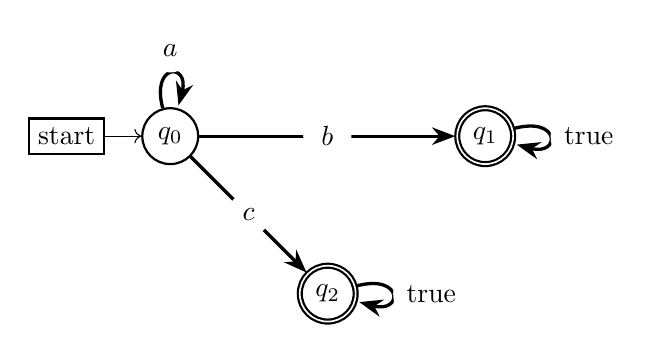
\begin{tikzpicture}

      \begin{scope}[every node/.style={circle,thick,draw}]
        \node[initial] (q0) at (-2, 2) {$q_0$};
        \node[accepting] (q1) at (2, 2) {$q_1$};
        \node[accepting] (q2) at (0, 0) {$q_2$};
      \end{scope}
      
      \begin{scope}[>={Stealth[black]},
          every node/.style={fill=white,circle},
          every edge/.style={draw=black,very thick}]
        \path [->] (q0) edge[loop above] node {$a$} (q0);
        \path [->] (q0) edge node {$b$} (q1);
        \path [->] (q0) edge node {$c$} (q2);
        \path [->] (q1) edge[loop right] node {true} (q1);
        \path [->] (q2) edge[loop right] node {true} (q2);
      \end{scope}
    \end{tikzpicture}
        \end{center}
    \hfill(5pts)

    \textbf{Answer:} The satisfying LTL formula $\lu{a}{(b \lor c)}$. 
$\lu{a}{(b \lor c)}$ holds in this Automata because it satisfies b or c to reach the final state, and it can loop in state $q_0$ using $a$ any number of times. Once it reaches the final state, it satisfies $\lu{a}{(b \lor c)}$, and after that, we do not care.  Therefore, it satisfies $\lu{a}{(b \lor c)}$
    
    
  \item \textbf{512 Question. Extra Credit for 412.}  Automata $A_2$
  (\emph{Hint: Look closely at the states $q_0$ and $q_1$. What
  type of patterns over $a$ and $b$ originate from $q_0$ and $q_1$?})
    \begin{center}
    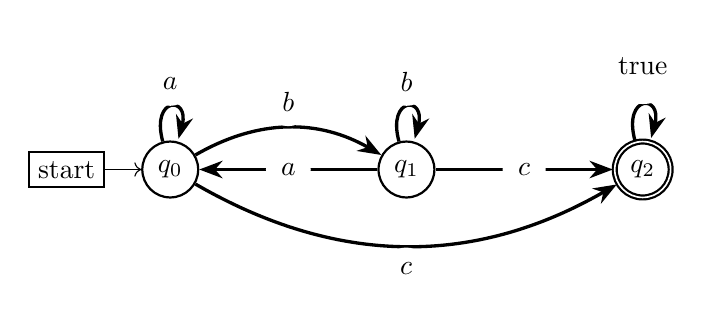
\begin{tikzpicture}

      \begin{scope}[every node/.style={circle,thick,draw}]
        \node[initial] (q0) at (0, 0) {$q_0$};
        \node (q1) at (3, 0) {$q_1$};
        \node[accepting] (q2) at (6, 0) {$q_2$};
      \end{scope}
      
      \begin{scope}[>={Stealth[black]},
          every node/.style={fill=white,circle},
          every edge/.style={draw=black,very thick}]
        \path [->] (q0) edge[loop above] node {$a$} (q0);
        \path [->] (q0) edge[bend left, above] node {$b$} (q1);
        \path [->] (q1) edge node {$c$} (q2);
        \path [->] (q1) edge node {$a$} (q0);
        \path [->] (q1) edge[loop above] node {$b$} (q1);
        \path [->] (q2) edge[loop above] node {true} (q2);
        \path [->] (q0) edge[bend right, below] node {$c$} (q2);
      \end{scope}
    \end{tikzpicture}
        \end{center}
\hfill(10pts)

     \textbf{Answer:} The satisfying LTL formula $\lu{(a \lor b)}{c}$. $\lu{(a \lor b)}{c}$ holds if $c$ holds immediately or all states along the path satisfies $a \lor b$ until it reaches $c$. In the Automata, starting from $q_0$, the states $q_0$ and $q_1$ can be visited any number of times using a or b, and once it goes to $q_2$, it finds $c$. So $\lu{(a \lor b)}{c}$ is satisfied in the Automata. 

     
    \end{enumerate}




\end{enumerate}


\end{document}

